\cleardoublepage
\chapter{System Architecture} \label{chap:sysArch}
%\todo[inline,color=yellow!40]{under review - v1.1 correcting last version}
%\todo[inline,color=blue!40]{*Chapter Introduction}
%\todo[inline,color=blue!40]{*1-System Elements}
%\todo[inline,color=blue!40]{     *1-The sensors/Actuator}
%\todo[inline,color=blue!40]{     *2-The processing Unit}
%\todo[inline,color=blue!40]{     *3-Processing type?}
%\todo[inline,color=blue!40]{*2-Architecture proposal}
%\todo[inline,color=blue!40]{*3-Approach to the problem}
Considering the techniques presented in the previous chapter~\ref{chap:stArt}, the one used in the development of the prosed solution will be the ~\citeauthor{wuAnalysisImplementationNoncontact2016a}\cite{wuAnalysisImplementationNoncontact2016a}. Their stimulation technique and corresponding captured signals are similar to what is itended to obtain, but using a different sensor to measure the vibration from the hammers impact. The details of their approach both theoretical and practical, are specified in section~\ref{sec:LPGModel}. This allows to better understand the details of the system and how to approach it. With this consideration and the previously presented studies, this chapter will dedicate its focus, on the presentation of the main elements of the system, and briefly explaining their function, aiming to aid in the definition of a raw architecture for the system, and in the interaction between elements within.

\section{System Elements}
In order to develop a system that is able to properly measure and return an good approximation of the liquid level in the LPG bottle, it is necessary to identify the elements that must be present in the system.

\subsection*{Actuator}
It is element responsible for the stimulation of the system. The main function of the actuator is to induce a transversal vibration throughout the system. In the presented work, two different techniques are proposed.
\subsection*{Sensor}
The variety of sensors that can be used to measure vibration, not specific to this case only, is very wide. When choosing a specific one, it must be taken into consideration aspects like its practical application. More specifically, the dimensions of the sensor, its cost and the physical coupling between the system to be measured and itself, as an example. Other electrical aspects to be taken in consideration, are specific to the type of sensor itself and may vary from one to another.

\subsection*{The Processing Unit}
The selection of the processing unit is quite important, since it is the ”brain” of the entire system. Firstly, it is responsible for the interaction between sensors, actuators and with the rest of the system. It is also where the gathered data is processed and how the resulting information is returned to the user. In this particular application, it returns a data corresponding to the measured to the liquid level.

To achieve this, the processing unit must be equipped with different types of I/O ports, and, most importantly, the ADC, for converting the continuous time signal to a discrete signal. Besides the I/Os, the system must have the computational power to perform any type of mathematical tasks needed in the signal processing. This does not mean it must include dedicated DSP hardware, but it should be able to perform those tasks in a reasonable period of time.

 
%Not sure if it should be here
\subsection*{Processing Architecture}
%\todo[inline,color=red!40]{Should be here?}
As a signal is converted and stored in the processing unity, it is decomposed into two variables. The dependent is usually related to the amplitude of the signal, and the independent with the sample, and overall can be seen as the output of a sensor at a certain moment of time. While this data can be used to return visual information about the state of the sensor, it is not the only way. Usually, the frequency spectrum is used to identify patterns in the system’s response that are not clear in time domain.

\section{Architecture proposal} 
The system architecture consists in the union of the mentioned elements, as to obtain a device capable of measuring what is intended. The device itself should be attached to each \acrshort{lpg} bottle, and be able to return to the user the level of liquid inside. The figure~\ref{fig:systemArch} is an illustration of the system’s elements.

\begin{figure}[]
    \centering
    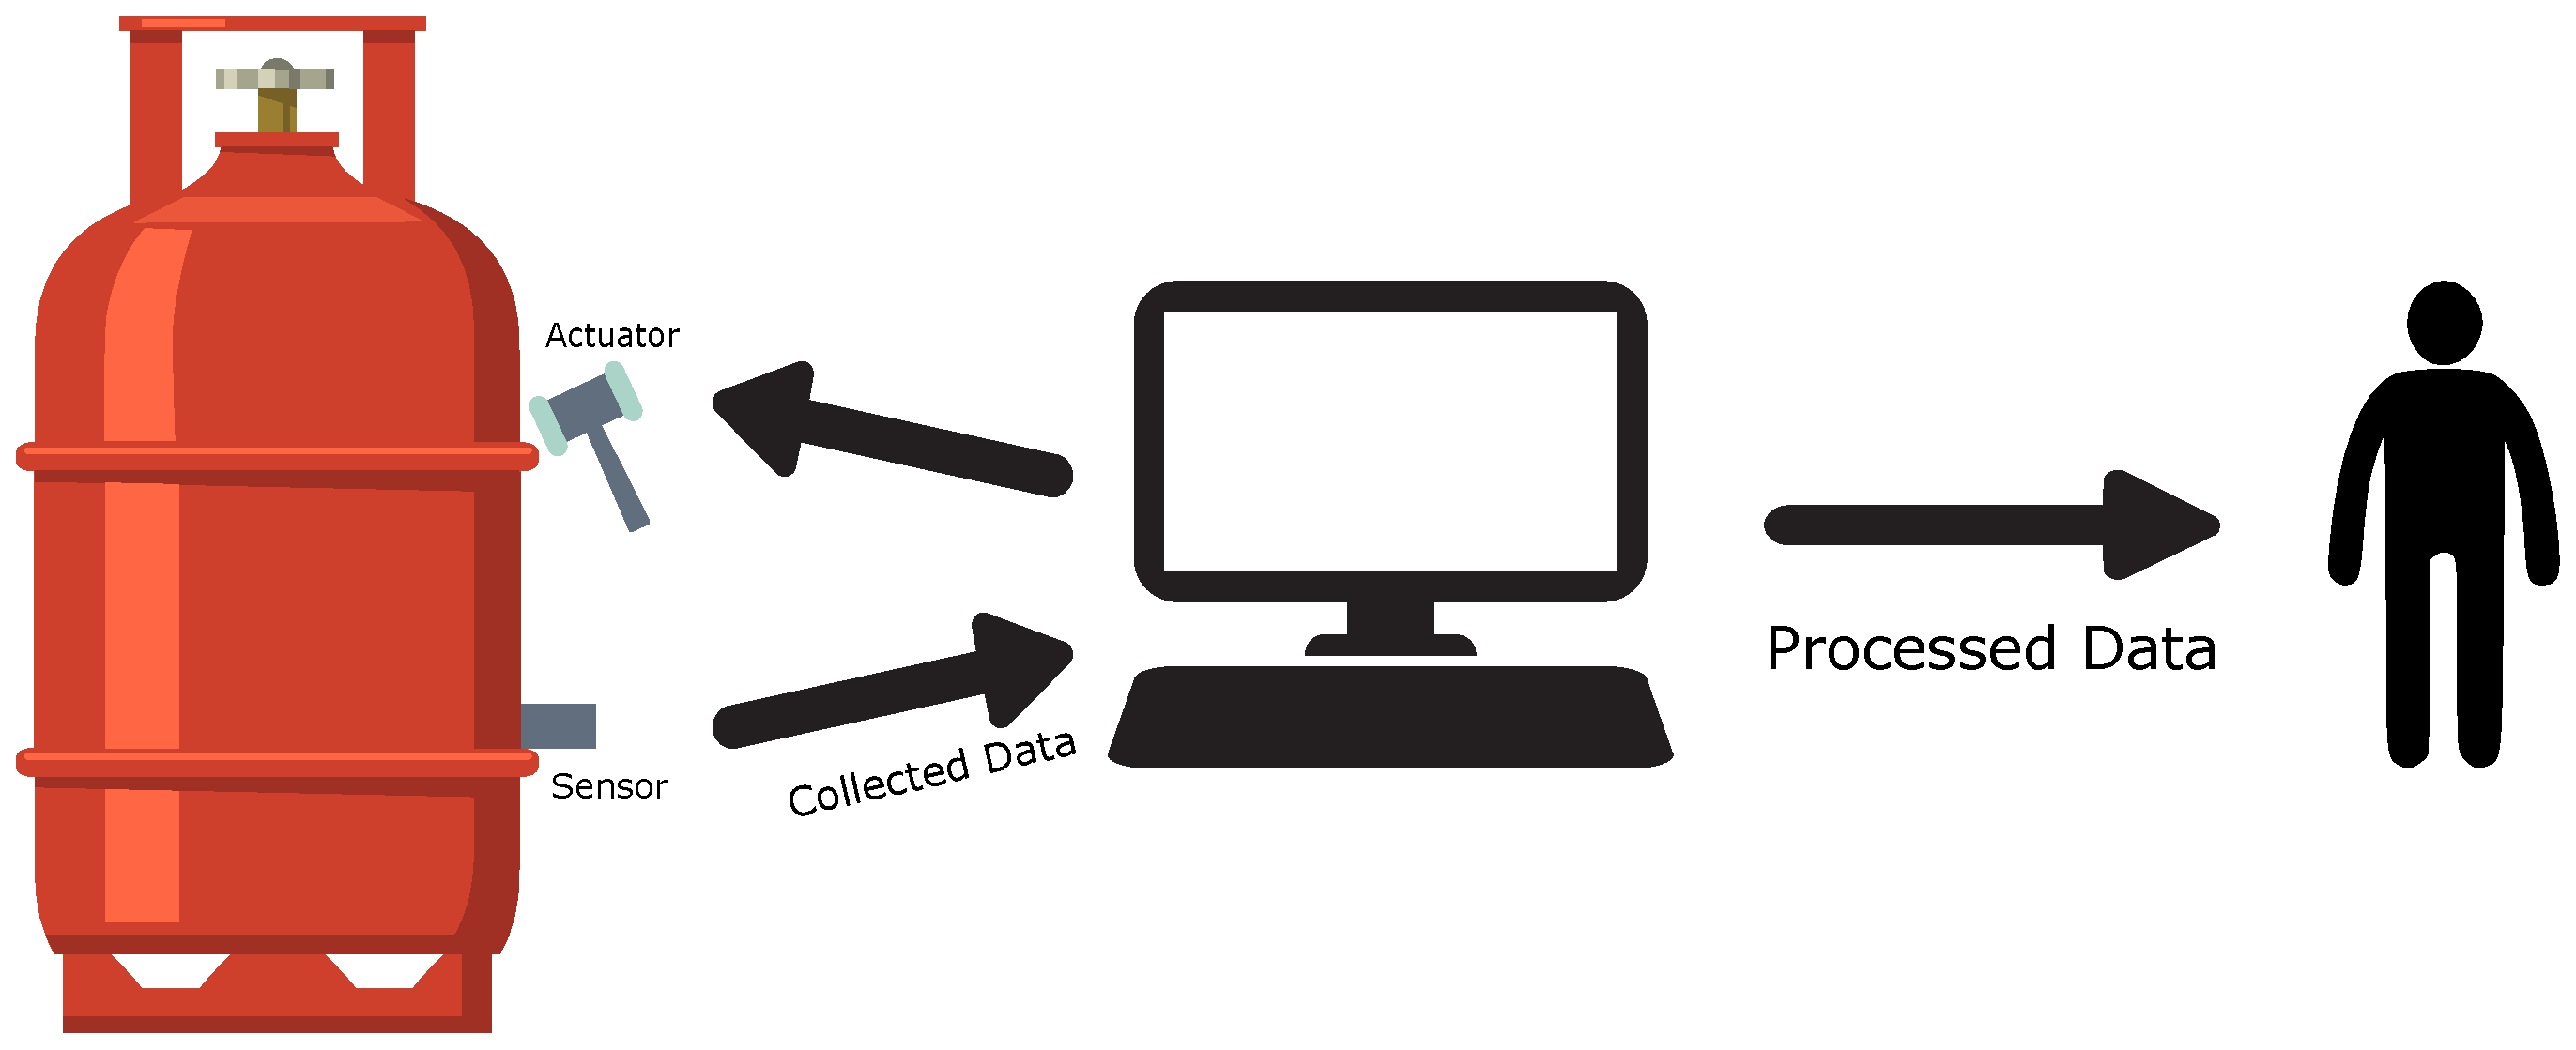
\includegraphics[width=0.55\textwidth]{Chapters/3CHP/Images/bottleBaseAct.eps}
    \caption{Basic architecture of the liquid level measuring device}{}
    \label{fig:systemArch}
\end{figure}

As mentioned previously, the processing unit is responsible for the control of the system. Firstly, it is responsible for triggering the actuators which, in this case, corresponds to the hammer hitting the side surface of the LPG bottle, producing the vibration. In the mean time, the processing unit starts to convert the signal from the sensor, to and store the value. Then, the recorded data must be processed, in order to return to the user the desire information. Ideally, this procedure would occur once or twice a day, unless a manual measure was requested by the user. But for the purpose of this work, the main purpose is to get information, and be able to associate it to a volume of liquid in the bottle.

The chosen method to process the information, is through the analysis of the acquired data in the frequency domain. To achieve that, a \acrshort{fft} used to process the gathered data, and afterward associate it to a given level of liquid. A brief and visual description of the flow of how the process occur’s in the processing unit is illustrated in figure~\ref{fig:systemSWFlow}.

\begin{figure}[]
    \centering
    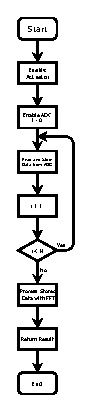
\includegraphics[width=0.15\textwidth]{Chapters/3CHP/Images/fluxogramArchProp.eps}
    \caption{Proposed diagram for the device operation}{}
    \label{fig:systemSWFlow}
\end{figure}
%\todo[inline,color=red!40]{Should I explain the diagram, or isn't necessary from the explanation before the ilustration?}

\section{Problem Approach}
The approach to obtain a solution and hopefully a device capable of measuring correctly the LPG liquid level will be split into two main phases. The first one is the study of the behavior of the system to an external stimulation, followed by the development of the solution for this case. In both phases the hardware selection will differ. In the first stage, MatLab is used in the data processing. This
system allows for easy manipulation of several of the system’s parameters, like the maximum and minimum volume of liquid. Besides it allows to develop a solution without compromising its performance due to hardware limitations, due to established FFT algorithms.

The second stage will be divided in several smaller steps, so it is possible to individually address any source of problems. In this stage, the microphone will be replaced with two sensors. Besides, the hammer previously used continue to be implemented as a stimulation method, being later replaced with a solenoid, in order to automatically perform the trigger and posterior signal acquisition. Similarly, in the beginning, MatLab also used to process the data, but it is later replaced by a microcontroller. The reason for this is that it is easier to understand
the type of signals acquired from the sensors and the proper way to process this data later, on the hardware implementation, avoiding skipping steps.
\section{End of chapter considerations}
From the identification of the elements of the system, it is possible to define an approach to the problem presented, this chapter focuses exactly on that. Knowing those elements we are able to start to work in each element in order to integrate them in the final solution. The following two chapters will be dedicated to explore each element individually, they will be divided in two to separate the hardware/physical elements from the software.

\clearpage
%\printbibliography[heading=subbibliography]
%\addcontentsline{toc}{section}{References}